
\documentclass{sig-alternate-05-2015}

% The following \documentclass options may be useful:

% preprint      Remove this option only once the paper is in final form.
% 10pt          To set in 10-point type instead of 9-point.
% 11pt          To set in 11-point type instead of 9-point.
% authoryear    To obtain author/year citation style instead of numeric.

\usepackage{amsmath}
\usepackage{url}
\usepackage{subfigure}
\usepackage{listings}
\usepackage{eqnarray}

\usepackage{graphicx}
\usepackage{algorithm}
%\usepackage{algorithmic}
\usepackage{algpseudocode}% http://ctan.org/pkg/algorithmicx
\usepackage{amsmath}
\usepackage{mathtools}
\usepackage{caption}
\usepackage{diagbox}

\graphicspath{{./Figures/}}

\algdef{SE}[DOWHILE]{Do}{doWhile}{\algorithmicdo}[1]{\algorithmicwhile\ #1}
\algnewcommand{\LeftComment}[1]{\Statex \(\triangleright\) #1}

\begin{document}

\setcopyright{acmcopyright}

\conferenceinfo{XXXX 'XX}{Month d--d, 20yy, City, ST, Country}
\acmPrice{\$15.00}

% Uncomment one of the following two, if you are not going for the
% traditional copyright transfer agreement.

%\exclusivelicense                % ACM gets exclusive license to publish,
                                  % you retain copyright

%\permissiontopublish             % ACM gets nonexclusive license to publish
                                  % (paid open-access papers,
                                  % short abstracts)

%\titlebanner{}        % These are ignored unless
%\preprintfooter{}   % 'preprint' option specified.

\title{Demystify Microarchitecture in GPU to Tune SGEMM Performance}
\subtitle{}


\maketitle

\begin{abstract}
	In this paper, we present thorough experience on tuning single precision general matrix multiplication (SGEMM) in assembly level on NVIDIA GPU architecture. First, we propose a methodology to demystify GPU's microarchitecture level optimizations. An instruction solver is developed to retrieve the undocumented ISA specification, which enables us to build an assembler that generates CUDA binary compatible files. We further design a rigorous microbenchmark to identify four microarchitectural features of control functions, register allocation, arithmetic throughput, and memory operations. Second, we tune SGEMM by applying the correlated microarchitectural optimizations, which go through the architecture hierarchy including maximizing FFMA throughput (core), eliminating register bank conflict (register), and selecting data path to shared/global memory (memory). The optimized SGEMM achieves the maximal floating-point efficiency of 88\%, which are 25\% higher than CUBLAS's 63\% on a NVIDIA Kepler GPU.
\end{abstract}

%\category{CR-number}{subcategory}{third-level}

% general terms are not compulsory anymore,
% you may leave them out
%\terms
%term1, term2

\keywords
SGEMM, Assembler, GPU, Performance
\section{Introduction}
Single Precision General Matrix Multiply (SGEMM) performs a multiplication of two single-precision matrices and is one of the basic routines in BLAS library~\cite{blas}. It has been extensively used in many scientific and engineering computing applications. Recently, SGEMM has drawn increasing efforts on performance tuning since it is the performance critical kernel in deep learning applications~\cite{chetlur2014cudnn,nervana_sgemm_wiki}.

As GPU provides higher peak FLOPS over CPU contemporarily, people tend to adopt GPUs to accelerate such a floating-point intensive computation. In fact, SGEMM's performance highly relies on low-level microarchitecture features. Hardware
vendors provide BLAS libraries tuned on their own processors, e.g. MKL/ACML~\cite{intel2007intel,amd2014} for multicore x86 CPUs and CUBLAS/CLMath~\cite{nvidia2008cublas, clmath}for
GPUs. However, we always witness improvement from third-party implementations over these vendors' libraries. For
multicore CPUs, based on hand-tuned assembly codes, OpenBLAS~\cite{xianyi2012openblas} achieves the best performance in most cases.
Although there is a lack of an OpenBLAS-like library on GPUs, several ongoing efforts~\cite{tan,lai,nervana_sgemm_wiki,
chien, volkov} achieve better performance than CUBLAS for either SGEMM or DGEMM by tuning assembly codes. However, these scattered works remain two issues to be addressed to accomplish the microarchitecture based performance tuning on each generation of GPUs.

\begin{itemize}
\item {\em There is a lack of a toolchain to identify GPU microarchitecture features and guide performance tuning.}
    Unlike general-purpose CPU community where a series of toolchains are available to tune performance in a bare metal
        way, only the abstract CUDA model is encouraged. A major reason is the significant changes of GPU architecture
        between each generation. For example, graphic features, register bank conflicts, and floating-point instructions dual
        issue of the recent ISA are totally different from the previous generations~\cite{fermi}. Fortunately, people have made
        some initial progress on performance tuning tools due to the pursuit of extreme performance, including
        benchmarking~\cite{mei, volkov, wong} and disassembler~\cite{asfermi,bernstein2012usable,decuda,maxas} on a specific GPU architecture. We attempt to develop a methodology that provides a systematic way to identify microarchitecture by decoding instruction formats automatically, generating ISA-compatible executable codes and benchmarking.
\item {\em There is a lack of a comprehensive understanding of SGEMM's performance in terms of low-level GPU microarchitecture.} Most SGEMM analyses are circumscribed at the levels of either CUDA or PTX because there is short of bare-metal tools on GPUs. Unfortunately, these analyses cannot directly diagnose either compiler deficiency or hardware defect. In fact, by observing the disassembled code of SGEMM in CUDA, we find that the generated control code is very inefficient in exploiting {\tt FFMA} dual issue (See Figure~\ref{fig:assemblycode} in section~\ref{sec:optimization}). It indicates that NVCC generated code does not completely utilize $192$ cores on an SM (streaming processor), leaving them idle at most of the time. A side effect of the limitation leads to a bias estimation of performance bound. We present a thorough analysis of performance which goes through the whole architecture hierarchy, including instruction throughput, register allocation, and shared/global memory transactions. The understanding of microarchitecture helps us build a robust performance model of SGEMM.
\end{itemize}

In this paper, we crack instruction encoding by performing a tough reverse engineering work, and then build an assembler to generate CUDA binary files. Because of the compatible grammar of CUDA {\tt cuobjdump}~\cite{cubin2015util}, we use CUDA toolchains~\cite{nvcc} to compile CUDA codes to a {\em cubin} file and then disassemble it to generate assembly codes. This approach supports users to optimize any code segment on the base of generated codes instead of coding from scratch. By using this assembler, we design a set of microbenchmarks that demystify lots of GPU microarchitecture details such as instruction issue, warp schedule, register bank distribution, and control code, which are helpful to understand and optimize the performance of SGEMM. We apply a collection of optimizations to improve SGEMM performance incrementally. More specifically, we make the following contributions:
\begin{itemize}
\item We propose a reverse engineering approach to crack the instruction encoding of GPU architecture, especially for control codes that orchestrate instruction scheduling. An assembler is developed to directly tune the assembly codes generated by CUDA compiler.
\item We design a bunch of benchmarks to reveal microarchitectural features which are undocumented by NVIDIA. They are necessary to understand and tune the performance of GPU programs.
\item We implement the highest performance SGEMM routines on NVIDIA Kepler by applying the demystified microarchitecture-level optimizations. The optimized SGEMM achieves the maximal floating-point efficiency of 88\%, which is 17\% higher than CUBLAS.
\end{itemize}

Although this work demonstrates the effectiveness on NVIDIA Kepler architecture, the approach is general-purpose for other NVDIA GPU architectures by minor adjustments of instruction solver and benchmarking. To the best of our knowledge, it is the first time to provide a detailed description of how to crack the instruction encoding for NVIDIA GPUs~\footnote{We'll open the sourcecodes to public in GitHub after the double-blind review.}. The experience of exploring bare-metal optimizations is valuable to compiler developement and performance tuning.

The rest of this paper is organized as follows. Section~\ref{sec:background} introduces the CUDA binary utilities and a blocking SGEMM algorithm. Section~\ref{sec:assembler} presents the instruction solver algorithms and microbenchmarking insights. Section~\ref{sec:optimization} applies a series of microarchitectural optimizations to SGEMM. We report experimental results on section~\ref{sec:experiment}. Section~\ref{sec:related} summarizes the related work. Finally, section~\ref{sec:conclusion} concludes this work. 

\section{Background}
\label{sec:background}
Since we seek to optimize SGEMM at assembly-level, this section introduces some CUDA binary utilities used in our work. Besides, we highlight tunable factors that determine SGEMM's performance on GPU architecture.

\subsection{CUDA Binary Utilities}
\label{sec:cuda}

A CUDA binary file, also called {\em cubin}, is an ELF-formatted file generated by CUDA compiler ({\tt nvcc}). It can be either embedded into a host executable file or generated separately by using the "{\em -cubin}" option of {\tt nvcc}. To help developers understand {\em cubin} files, CUDA toolkit introduces binary tools and documents on ISAs from GT200 to Maxwell architecture~\cite{gtx980}. These binary tools only provide very limited functionalities for users. For instance, both {\tt cuobjdump} and {\tt nvdiasm} disassemble {\em cubin} files to {\em sass} files, which are readable assembly codes for examining possible performance issues in GPU programs. For each instruction in the executable code sections, the tools list its address in hexadecimal, mnemonics in string, and encoded number in hexadecimal. For example, an {\tt IADD} instruction might be printed as follows: \\\\
$/*0048*/~~~~IADD~~R0,~~R2,~~R0;~~/* 0x4800000000201c03 */$\\\\
Unfortunately, these tools do not enable us to modify the assembly codes directly for tuning performance. What we can do is to refine CUDA C codes after examining the read-only assembly codes iteratively. Therefore, an assembler is required to manipulate assembly codes. Although NVIDIA does not release its internal assembler and instruction encoding format, the disassembled code and the released pseudo assembly references~\cite{ptx2015isa}, provide us clues to crack instruction format (in Section~\ref{sec:assembler}).


\subsection{Performance Factors of SGEMM}
\label{sec:sgemm}
It's well-known that the primary factors of SGEMM performance are the blocking parameters for exploiting data reuse through memory hierarchy. On GPUs, we should consider both shared memory blocking and register blocking. For the purpose of completeness, we describe a blocking algorithm which is similar to that in other literature~\cite{magma,nervana_sgemm_wiki,lai,tan}.

Algorithm~\ref{gemm} shows the skeleton of SGEMM blocking algorithm. Task partition is based on the result matrix $C$. Each thread block with $tx*ty$ threads is responsible to compute a $bm*bn$ submatrix in $C$, where $bm, bn$ are the number of rows and columns of the submatrix, respectively. We need read a $bm*bk$ from A and a $bk*bn$ sub-matrix from B for each thread block, where $bk$ is unroll factor. In this way, $A$, $B$ and $C$ are divided into $M*K$, $K*N$ and $M*N$ grids of $bm*bk$, $bk*bn$ and $bm*bn$ blocks, where $M=\Bigl\lfloor \frac{m+bm-1}{bm} \Bigr\rfloor$, $K=\Bigl\lfloor \frac{k+bk-1}{bk} \Bigr\rfloor$, $N=\Bigl\lfloor \frac{n+bn-1}{bn} \Bigr\rfloor$.

\begin{algorithm}
  \caption{SGEMM blocking algorithm. {\em smA} and {\em smB} are shared memory variables. {\em rA}, {\em rB} and {\em accum} are register variables. $rx$ and $ry$ are register blocking sizes}
  \label{gemm}
  \begin{algorithmic}[1]
	\LineComment {The size of a thread block: $tx*ty$}
	\LineComment {Registers: accum[$rx*ry$], rA[$2*rx$], rB[$2*ry$]}
	\State $smA[bm][bk] \gets$ a $bm * bk$ block of $A$
	\State $smB[bk][bn] \gets$ a $bk * bn$ block of $B$
	\Do
      \For {{$i \gets 1, bk$}}
      %\Comment {\color {mygray} {Unrolling for loop}}
      \Comment {{Unrolling for loop}}
      \State {\color {black} {$rA[0...rx]\gets$ a column of $smA$}}
	\State $rB[0...ry]\gets$ a row of $smB$
	\State $accum[0...rx][0...ry]\gets accum[0...rx][0...ry]+rA[0...rx]*rB[0...ry]$
	\EndFor
	\State $smA[bk][bm]\gets$ a $bm*bk$ block of $A$
	\State $smB[bk][bn]\gets$ a $bk*bn$ block of $B$
	\State \textbf{sync}
	\doWhile {pointer in $B$ is out of range}
	\State \textbf{merge} $accum[0...rx][0...ry]$ with a $bm*bn$ block of $C$.
  \end{algorithmic}
\end{algorithm}

The volume of float point computations inside the while loop of Algorithm~\ref{gemm} is $2\times rx\times ry \times bk$ in operations, and Table~\ref{tab:reg} estimates data movement volume through registers, shared memory, and global memory for each threads inside while loop.
These parameters demonstrate that SGEMM performance is affected by the hierarchical memory blocking and unrolling factors in the inner loops.
The tuning of these factors is conducted in two folds--memory bandwidth and latency. In fact, with the estimations in Table~\ref{tab:reg}, it is relatively easy to tune proper parameters to eliminate the bound of memory bandwidth~\cite{magma}~\cite{tan}. The difficulty lies in latency, which is closely related to specific microarchitectures such as instruction sequence, instruction type and so on. However, the microarchitectural optimizations depend on the availability of an assembler and deep understanding of microarchitectural features. %TODO the second last sentence

\begin{table}[!t]
\caption{Data movement volume of each thread inside while loop}
\centering
\scalebox{1.0} {
\begin{tabular}{|c|c|}
\hline
    Data path& Volume(in words)\\
\hline
    global$\Rightarrow$regitster ({\tt LDG})& $\frac{rx*\times ry \times bk}{bm} + \frac{rx\times ry \times bk}{bn}$ \\
\hline
register$\Rightarrow$shared ({\tt STS})& $\frac{rx*\times ry \times bk}{bm} + \frac{rx\times ry \times bk}{bn}$ \\
\hline
shared$\Rightarrow$register ({\tt LDS})& $rx\times bk + ry\times bk$\\
\hline
%    arithemtic({\tt FFMA})& $rx\times ry \times bk$\\
%\hline
\end{tabular}
}
\label{tab:reg}
\end{table}

\section{Demystify Microarchitecture Features}
\label{sec:assembler}

\subsection{Methodology}
We propose a methodology to demystify GPU microarchitecture features and correlate them with performance. The workflow consists of three components: CUDA binary tools, a instruction solver, and a rigorous microbhenchmark. We leverage CUDA binary tools to generate assembly codes for sample programs or libraries. A sample program is a synthetic CUDA file targeted to generate some specific instructions. A library might provide a high coverage of instruction sets. For example, the CUBLAS library contains almost all instructions used in SGEMM routines. As introduced in section~\ref{sec:cuda}, these generated assembly files ({\em sass}) provide a instruction encoded number to be cracked.

The instruction solver takes the assembly files as input to decode 64-bits binary representation of each instruction. We design a set of algorithms to solve all fields of the binary instruction. These fields include {\em register, predicate, address, immediate, constant} and {\em opcode}. The solver retrieves the undocumented ISA specification, which is used to implement an native assembler. Then, we design a rigorous microbenchmark and leverage the assembler to tune code at assembly language level. In the end, the tuning process will lead to some practical observations on the correlation between microarchitecture and performance.

\begin{figure}[htbp]
\begin{center}
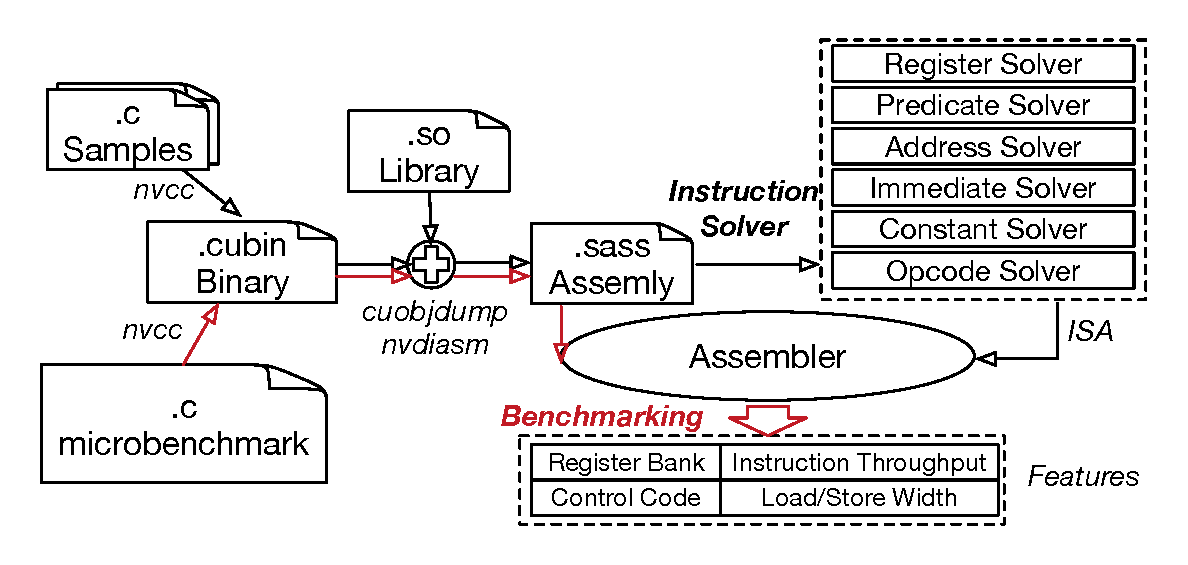
\includegraphics[scale=0.45]{methodology}
\caption{A schematic diagram of demystifying GPU microarchitecture features by leveraging CUDA binary tools. The back arrows represent the workflow of instruction solver while the red ones represents that of benchmarking to find out correlation between microarchitecture and performance.}
\label{fig:workflow}
\end{center}
\end{figure}

\subsection{Instruction Solver}
An instruction is composed of three fields: {\tt opcode}, {\tt operands} and {\tt modifiers}. An operand can be register, constant memory, global memory, shared memory, immediate, or predicate register.
The encoding of operands can be inferred by their names. For instance, the register operand {\tt R5} could be
inferred as $101$ in binary format, immediate $0x9$ is represented as $1001$. Besides, the fixed lengths of these fields allow us to determine their positions and lengths and hence encoding. Encodings of opcode and modifier are mnemonic symbols, we can not infer encoding by their names. Modifiers are instruction specific, the same kind of modifier can be different encodings for different instructions. For instance, mask of type-size
modifier for {\tt LD} and {\tt LDG} are at different positions. So we deal with modifier for each instruction separately.

\subsubsection{Operands:Fixed Length Field}

The basic idea of Algorithm~\ref{algo:int_solver} is that match binary encoding of operand in $64$ instruction encoding and find
position until the postion is unique. The input instructions are from disassembly code (i.e., NVIDIA CUBLAS library).
First, we randomly pick up instruction that has the filed we want to probe, and represent it in binary by its name. Second, we match its binary in $64$-bit instruction encoding, and find possible positions. Third, we intersect current candidate with previous one, if the number of candidate is $1$, we find the position. Otherwise, we set the current candidate to the previous one and randomly pick next instruction to repeat the procedure.

\begin{algorithm}
      \caption{Solver}
      \label{algo:int_solver}
  \begin{algorithmic}[1]
	  \State \textbf{input:} instmap
      \State output: pos, length
      \State currpos=\{\}
      \State prepos=\{0,1,2,...63\}
      \While {lenght(currpos) != 1}
      \State inst=instmap[random()]
      \If {inst.src1type == immediate}
      \State instencode=inst->encode64bit
      \State immbin = completecode(imm)
      \State pos = 0
      \While {pos + length(immbin) < 64}
      \If {strcmp(immbin,instencode+pos,length(immbin)}
      \State pushback(currpos, pos)
      \EndIf
      \EndWhile
      \State currpos = intersect (curpos, prepos)
      \State prepos = currpos
      \State currpos=\{\}
      \EndIf
      \EndWhile
      \State return curpos[0]
  \end{algorithmic}
\end{algorithm}


After finding the operand position, we need to infer or veritify the length of operand encoding. Some are easy to be
inferred, for example, there are at most $256=2^{8}$ registers for each thread, we could infer the length of register operand to be $8$.
The others like immediate or script note of constant memory is more complicated. One solution is to set the bit from the
position one by one to check whether the operand value is grown as we expected.

\subsubsection{Opcode}
Opcodes does not show their encoding literally. One possible way is to write instruction {\tt PTX} code with flags
combinations based on syntax on NVIDIA PTX manual, and generate encoding by using NVDIA toolchain.
Then, opcode can be got by stripping out operand mask, and flags can be found by stripping out opcode and operand mask. However, the uncompleteness of NVIDIA document hinder us to find out all the opcodes and instruction modifiers. Another feasible way is to emulate all of possible binary combinations after striping out operand mask.
Normally, each instruction have $3$ register operand, and one $4-bit$ predicate register, we have $64-8*3-4=36$ bits left to probe.
In fact, we can further prune the search space by recognizing possible position by algorithm~\ref{algo:opcode}. By randomly probing bit by bit, we find that the top $10$ bits and lower $2$ bits represent opcode and other bits represent flags. Thus, we only enumerate these opcode bits which generate a acceptable search space. Finally, we find the minimal opcode without any flags. 


\begin{algorithm}
      \caption{Opcode Solver}\label{algo:opcode}
  \begin{algorithmic}[1]
      \State for each instruction in PTX generated database
      \For {i=0; i < num\_inst; i++}
      \For {j=0; j < 64; j ++}
      \If {isoperand(encode[i][j] == 0) and encode[i][j]== 0}
      \State newcode = encode[i][j].setbit(j, 1)
      \State newinst=nvdisasm(newcode)
      \If {sameop(newinst,oldinst) == 0 and isvalid(newinst) }
      \State pushback(j)
      \EndIf
      \EndIf
      \EndFor
      \EndFor
  \end{algorithmic}
\end{algorithm}

\subsubsection{Modifier: Instruction Specific}

Modifier defines a specific behavior for some instruction. For example,
{\tt LD} instruction has type-size modifiers, such as .u8, .s8, .u16, .32, .64 and .128. {\tt LD} also has cache operation modifier, such as .ca(cache at all level) and .cg(cache at global level). Modifiers (also called flags) are much more complicated because its position spans accross the reminding bits and one instruction may have more than one kinds of modifiers. By excluding both opcode and operand mask, there remain around $24$ bits. We observe that the default value for modifier is $0$. That is, modifier works when at least one bit is set. We can find possible positions of modifiers 
by greedily set the remaining bits one by one, the time complexity is $O(2^{10})$ instead of $O(2^{24})$. The number of bit is typically less
than $10$. After finding the candidates, we enumerate these bits, and group each kind.

\subsection{Correlating Microarchitecture with Performance}
With the assembler we tune the assembly codes of microbenchmark. According to the performance tuning results, we correlate microarchitecture with performance variants that guide performance optimizations in real applications. The correlation is presented as several meaningful observations, which are categorized into four microarchitectural features of {\tt control} function, {\tt register} allocation, {\tt arithmetic} throughput and {\tt memory} operation.

\begin{figure}[htbp]
\begin{center}
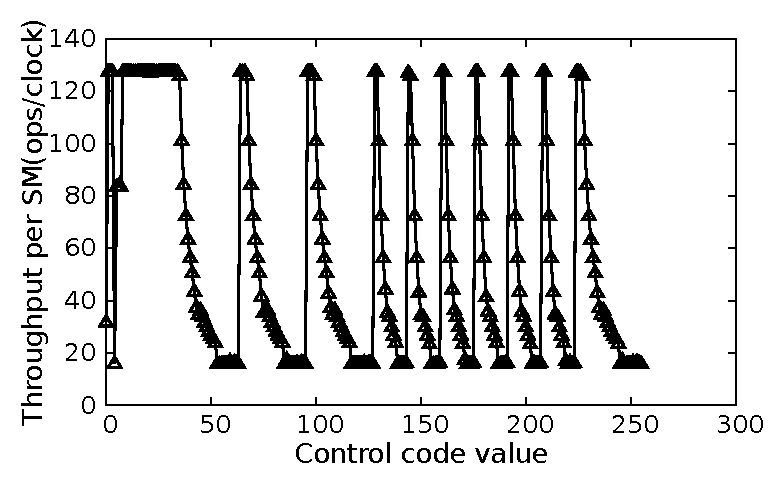
\includegraphics[scale=0.6]{ctrl}
\caption{Different control codes regulate {\tt FFMA} throughput.}
\label{fig:control_throughput}
\end{center}
\end{figure}

\begin{figure}[htbp]
\begin{center}
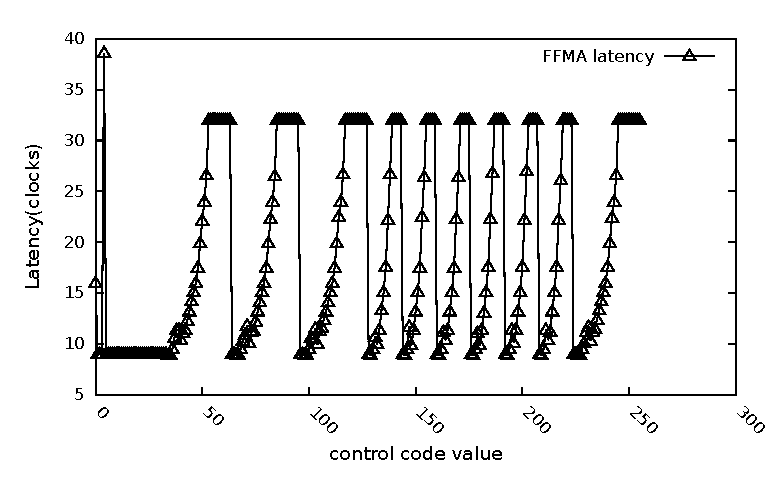
\includegraphics[scale=0.6]{ctrl_latency}
\caption{Different control codes regulate {\tt FFMA} latency.}
\label{fig:control_latency}
\end{center}
\end{figure}

\begin{figure}[htbp]
\begin{center}
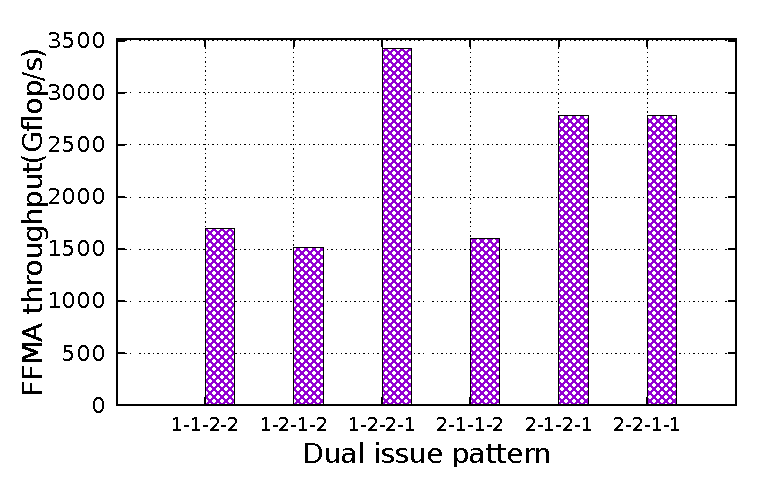
\includegraphics[scale=0.6]{pattern}
    \caption{Control codes pattern regulate peak {\tt FFMA} throughput(S:single issue, D:dual issue).}
\label{fig:pattern}
\end{center}
\end{figure}

{\em {\bf Observation 1--[Control]}: The execution sequence of instructions is regulated by control codes. Both warp scheduling and issue mode are tunable by setting control codes.}

Starting with the Kepler architecture NVIDIA has been moving some control logic off of the chip and into kernel instructions which are determined by the assembler. This evolution provides programmer a chance to make globally optimal decisions on scheduling and other control aspects if an assembler is available. The disassembly code indicates that every 64 bits control code controls $7$ instructions. We identify that both higher $6$ bits and lower 2 bits are {\em opcode} of control code, and the middle 56 bits are used to control the execution of $7$ instructions, each of which is assigned $8$ control bits.

For the eight control bits, we identify their meanings by examining CUBLAS disassembly codes and tuning a {\tt FFMA}
throughput microbhenchmark. We observe that the $7$th bit of the control code of {\tt TLD} instruction is $1$, which
indicates a texture dependency barrier due to weak consistent memory model. It's verified that some illegal values are
loaded if this bit is not set. Similarly, we discover that the $5$th bit means shared memory dependency barrier, the
$4$th bit means global memory dependency barrier. Figure~\ref{fig:control_throughput} shows that {\tt FFMA} throughput varies with all control bit values from 0 to 255. As shown in this figure, the throughput linearly decreases with the increasing values represented by the $0-3$ bits. That implies that these $4$ bits set the number of stall cycles before issuing the instruction. Further, the microbenchmarking reveal some specific patterns of control codes:

\begin{itemize}
\item When the control bits are set to be $0x40$, the scheduler suspends a warp of the instructions for 32 cycles.
\item $0x04$ means dual issue mode. If two consecutive instructions is controlled by $0x04$ and $0x05$, the throughput can reach the maximum. Single issue control code is $0x00$.
\item $0x20|n$ means a warp is suspended for $n$ cycles before issuing the next instruction, where $n$ is number between 0 and 15.
\end{itemize}


{\em {\bf Observation 2--[Register]}: Irrespective of single- or dual-issue mode, register bank conflict is only caused by source operands, and degrades instruction throughput by up to $17\%$.}

For CUDA programming model it is well-known that shared memory bank conflict is an important performance factor. In
fact, recent researches~\cite{lai} noticed that register bank conflicts are nontrivial to performance.  In order to probe register bank conflict, our microbenchmark measures instruction throughput for different combination of {\tt FFMA} register operands. Table~\ref{tab:th} shows an example of the combination which results in variance of efficiency. The numbers in the fifth column represent the number of registers conflict in the same bank. This experiment is conducted in single-issue mode by setting control code to be $0x20$. The theoretical efficiency is $128/192=66.67\%$. In fact, we observe that both single- and dual-issue mode produce the same variance of instruction throughput. Besides, from the experimental results we observe that:
\begin{itemize}
\item Destination operand will not contribute to bank conflict, no matter which bank is assigned to it.
\item When source operands have 2-way conflict, the throughput will drop by 2.33\% in single issue
    mode. When source operands have 3-way conflicts, the throughput will drop by 17.17\%.

 \item On Kepler architecture, our microbenchmark finds out a proper distribution of registers for eliminating bank
     conflict. The distribution is summarized in Table~\ref{tab:reg}, which confirms the follow the rule~\cite{lai}: \\
 bank0$\Leftarrow$($Rindex \% 8 < 4$ \&\& $Rindex \% 2 == 0$) \\
 bank2$\Leftarrow$($Rindex \% 8 < 4$ \&\&
$Rindex \% 2 == 1$) \\
bank1$\Leftarrow$($Rindex \% 8 > 4$ \&\& $Rindex \%2 == 0$) \\
bank3$\Leftarrow$($Rindex \% 8 < 4$ \&\&
$Rindex\% 2 == 1$)\\
where $Rindex$ is the register number. This rule will guide the performance tuning in the following SGEMM implementation.

\end{itemize}

\begin{table}[htbp]
\caption{The efficiency of instruction throughput varies with difference register bank distribution. {\it Inst} : instruction pattern, {\it Th/SM}: the instruction throughput per SM, {\it Eff}: efficiency of throughput.}
\centering
\scalebox{1.0} {
\begin{tabular}{|c||c|c|c|}
\hline
Inst &Th/SM&Eff&Conflicts \\
\hline
{\tt FFMA R5,R4,R1,R0}&127.50&66.40\%&0\\
\hline
{\tt FFMA R2,R4,R1,R0}&127.50&66.40\%&0\\
\hline
{\tt FFMA R5,R2,R1,R0}&119.18&62.07\%&2\\
\hline
{\tt FFMA R3,R2,R1,R0}&119.18&62.07\%&2\\
\hline
{\tt FFMA R5,R9,R3,R1}&94.52&49.23\%&3\\
\hline
{\tt FFMA R11,R9,R3,R1}&94.52&49.23\%&3\\
\hline
{\tt FMUL R4,R1,R0}&127.50&66.40\%&0\\
\hline
{\tt FMUL R4,R2,R0}&119.17&62.06\%&2\\
\hline
\end{tabular}
}
\label{tab:th}
\end{table}


\begin{table}[htbp]
\caption{Register distribution for zero bank conflict.}
\centering
\scalebox{1.0} {
\begin{tabular}{|c||c|c|c|c|c|c|c|c|c|}
\hline
Bank0&0&2&8&10&16&18&24&26&... \\
\hline
Bank1&1&3&9&11&17&19&25&27&... \\
\hline
Bank2&4&6&12&14&20&22&28&30&... \\
\hline
Bank3&5&7&13&15&21&23&29&31&...\\
\hline
\end{tabular}
}
\label{tab:reg}
\end{table}

{\em {\bf Observation 3--[Arithmetic]}: With a proper control code and register allocation, {\tt FFMA} instruction throughput can approach the theoretical peak in dual issue mode.}

It's very intricate to tune instruction execution to improve instruction throughput. The previous work report a maximal throughput of {\tt FFMA} on a SM is $132$, which is much less than the theoretical throughput $192$ on Kepler. Our microbenchmarks reveal several key points of optimization to approach theoretical peak on Kepler. First, the control code must be set properly to dual issue adjacent instructions. Second, the ratio and interval of dual issue {\tt FFMA} instructions must be tuned into a specific pattern. Since each warp of extra computing unit is shared among two warps, when all threads are trying to fully dual issue every two adjacent {\tt FFMA}s, half of the scheduler would stall due to computing resource conflict. The ratio of dual issue and single issue should be $2:2$, and with a proper phase shift among two warp's executing pace, they could get access to the shared computing unit in turn. Third, the first instruction of the core loop needs to be aligned. This restriction is caused by the aligned position of control code in the instruction sequence. Last, {\tt FFMA} dual issue requires 6 register banks. Instruction order has to be adjusted to fully use Kepler's operand collector mechanism to avoid register bank conflicts. As shown in Table~\ref{tab:ffma}, these optimizations together improve {\tt FFMA}'s throughput  to be $190$, which is very close to the theoretical peak $192$.

\begin{table}[htbp]
\caption{Floating-point instruction throughput on Kepler}
\centering
\scalebox{1.} {
\begin{tabular}{|c||c|c|c|}
\hline
Inst name&operation&single issue&dual issue\\
\hline
{\tt FFMA} &c=a*b+c&127.52&190.35 \\
\hline
{\tt FMUL} &c=a*b&127.52&190.35 \\
\hline
{\tt FADD} &c=a+b&127.52&192\\
\hline
\end{tabular}
}
\label{tab:ffma}
\end{table}


{\em {\bf Observation 4--[Memory]}: For achieving higher memory bandwidth, shared memory prefers to 64-bits load instruction {\tt LDS.64} while global memory prefers to 128-bits load instruction {\tt LDG.E.128} with texture path.}

For the GPU memory hierarchy we focus on the programmer controllable memory resources--shared memory and global memory. On NVIDIA GPU architecture, there are different memory access widths (i.e., 32-bits,64-bits,128-bits) and paths (i.e., normal cache or texture cache). In fact, both NVIDIA document and previous works~\cite{} pointed out that wider instructions have longer pipeline latencies, which are also measured in our microbenchmark. In addition, we identify several bandwidth issues for memory optimization.

Intuitively, a wider load operation achieves higher bandwidth. We benchmark bandwidth of shared memory operations {\tt LDS} with different widths, i.e., {\tt LDS.32}, {\tt LDS.64}
and {\tt LDS.128}. The operations are specially arranged so that no shared memory bank conflict occurs in a warp. In the
experiment, the amount of data are projected to the number of load instructions. For exmaple, if the data are loaded by
$N$ {\tt LDS.128} instructions, then either $2N$ {\tt LDS.64} or $2N$ {\tt LDS.64} instructions are required.
Figure~\ref{fig:lds_bw} compares the sequential memory access bandwidth with increasing volume of data. As shown in the figure, {\tt LDS.64} achieves the highest bandwidth $113GB/s$, which is about $60\%$ of the peak bandwidth\footnote{The theoretical shared memory bandwidth for each SM can be calculated as $Bandwidth=f_{core}*Width*Warpsize$ in
bytes, where $f_{core}$ is frequency of CUDA core, $Width$ is bank width, $Warpsize$ is warp size.}.

\begin{figure}[htbp]
\begin{center}
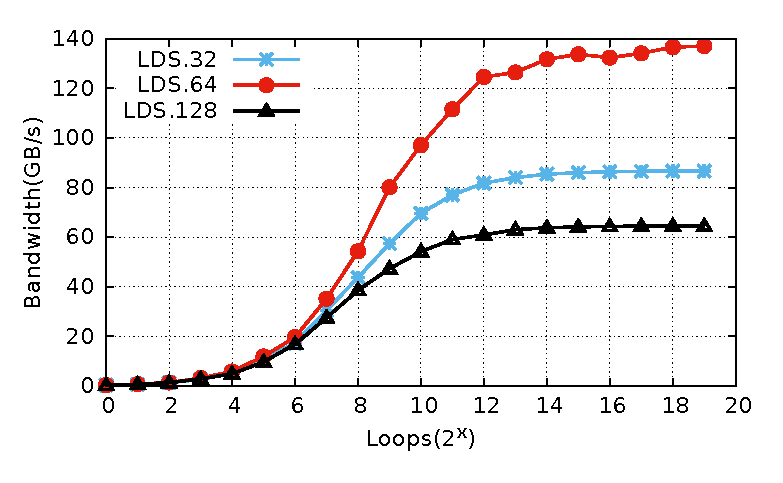
\includegraphics[scale=0.6]{lds_bandwidth}
    \caption{ Bandwidth of {\tt LDS.32}, {\tt LDS.64} and {\tt LDS.128}}
\label{fig:lds_bw}
\end{center}
\end{figure}

% global memory
There are two paths to global memory. One is from global memory to normal cache (L1 or L2), which is executed by {\tt
LD} instruction. The other one is from global memory to texture cache, which is executed by {\tt LDG} instruction. We
launche $26$ thread blocks with $512$ threads, and specifies that each thread access $4$ words with a stride of
$4*blockDim.x*gridDim.x$. Our benchmark confirms that {\tt LDG} achieves higher bandwidth than {\tt LD}, which has been
identified by previous work~\cite{tan}.

\section{Applying Optimizations to SGEMM\jled{Optimizing SGEMM}}
\label{sec:optimization}


The demystified GPU microarchitecture features provide a larger tuning space for computational kernels 
We apply
a series of incremental optimizations to improve SGEMM performance on Kepler architecture. The optimization strategies
go through architectural hierarchy from CUDA core and register to memory. All the optimization strategies are inspired by the observations from our benchmarking.
\begin{itemize}
\item At core level, we orchestrate {\tt FFMA} instruction executions with a more efficient instruction scheduling set by the proper control code.
% with respect to the proper control code pattern.
\item At register level, we meticulously map operands to registers so that bank conflicts are avoided for the inner loop in Algorithm~\ref{gemm}.
\item At memory level, we select appropriate shared memory load/store width and global memory data path to mitigate
latencies.
\end{itemize}

\subsection{Instruction Scheduling}
\subsubsection{Schedule {\tt FFMA} Instructions}
It's unrealistic to keep warp schedulers dual issue the same kinds of arithmetic instructions (i.e., {\tt FFMA}) all
the time. Because on Kepler architecture, each warp is assigned $32$ cores privately, $4$ warp schedulers will consume
$128$ cores. The reminding $192-128=64$ cores are divided into $2$ 32-core groups, each $32$ cores
are shared by $2$ warp schedulers. Two warp schedulers must negotiate who will use the extra $32$ shared cores to avoid
resource conflict.
As noted in {\em observation 3}, the best pattern of {\tt FFMA} instructions block is a sequence of $1$ single issue(1
{\tt FFMA}), 2 dual issues (4 {\tt FFMA}s) and 1 single issues ((1 {\tt FFMA})). As shown in
Figure~\ref{fig:assemblycode}, the instructions in lines 3-4 and lines 6-7 are dual issued separately.
The other two instructions in line 8 and line 11 are two single issues in terms of floating-point instruction
execution.
As a comparison, most of the {\tt FFMA}s are single issued in the CUDA compiler generated codes.

\begin{figure*}[htbp]
\begin{center}
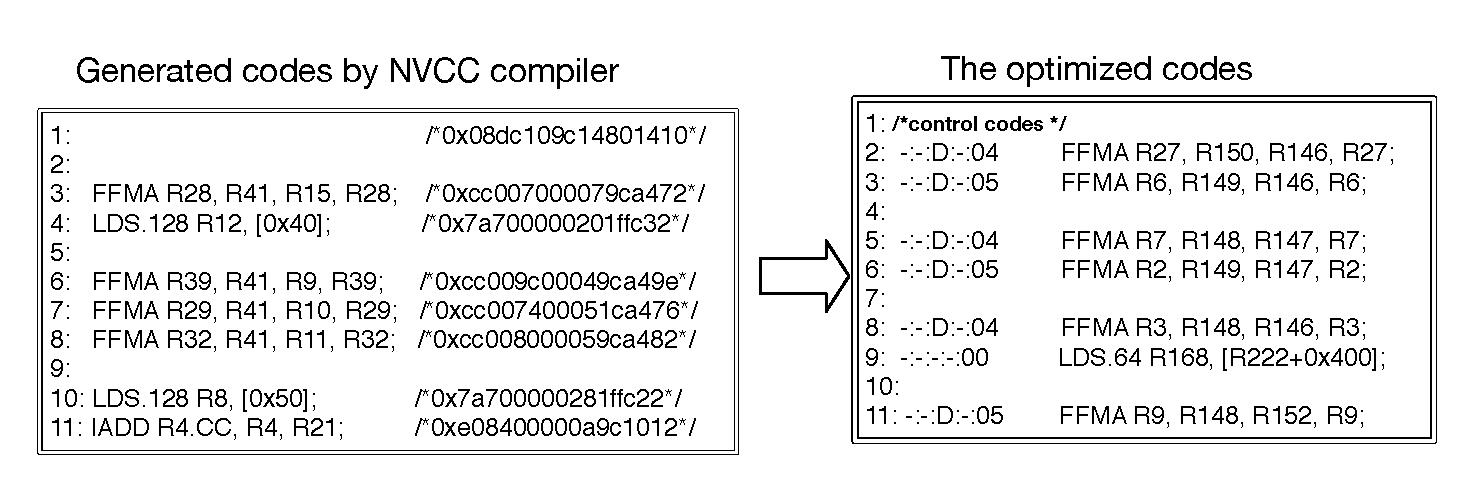
\includegraphics[scale=0.6]{assemlycode}
    \caption{The comparison of compiler generated codes and our tuned assembly codes.}
\label{fig:assemblycode}
\end{center}
\end{figure*}

\begin{figure}[htbp]
\begin{center}
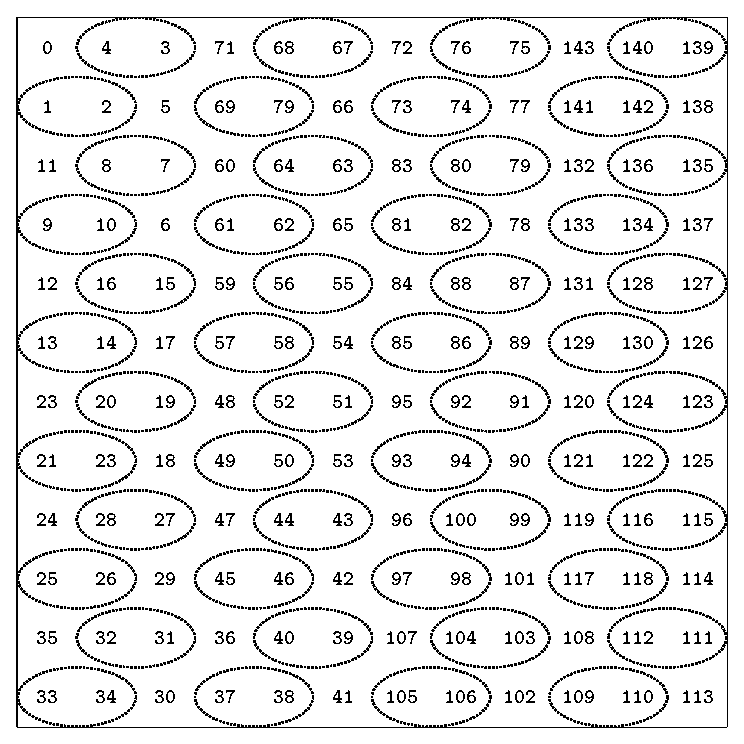
\includegraphics[scale=0.5]{order}
\caption{{\tt FFMA}s instruction scheduling to compute a $12\times 12$ sub-block of matrix C.  The numbers in
cells denote {\tt FFMA} execution order. Dashed ellipses across two cells mean that two {\tt FFMA} instructions are dual issued in one clock cycle.}
\label{fig:order}
\end{center}
\end{figure}

By extending the basic {\tt FFMA} $7$-instruction block (section~\ref{sec:benchmark}), we depict the scheduling pattern of computing a $12\times 12$ sub-block of matrix C in Figure~\ref{fig:order}.
% illustrates the order of $144$ {\tt FFMA}s instruction execution for calculating a $12\times 12$ subblock of matrix C.
For example, the {\tt FFMA} to calculate $c_{00}$ is issued first.
Then, two {\tt FFMA}s to
compute $c_{10}$ and $c_{11}$ are simultaneously issued. We arrange all the {\tt FFMA} instructions of SGEMM according to the order in Figure~\ref{fig:order}.

Another advantage of this execution order is less register pressure due to register reuse, which can facilitate
operand collector mechanism~\cite{collector}. Operand collector is a storage element coupled with register file and
provides inputs to the data path of the processor core for executing an instruction. \jled{This is not the first occurrence of Operand collector.} Operands may be cached and reused
in the subsequent instructions.
The assembly code in Figure~\ref{fig:assemblycode} lists the instructions to calculate $C_{32},C_{22}, C_{21}, C_{30},
C_{31}, C_{20}$, corresponding to the orders of $6,7,8,9,10,11$ in Figure~\ref{fig:reg}.
With the elaborately designed computing order and register allocation, the reuse happens as follows. The {\tt FFMA} in
Line $3$ uses cached operand {\tt R150} of line $2$, Line $3$ and Line $4$ share {\tt R146}. Thus, in dual issue mode
{\tt FFMA} of Line $3$ and $4$ need to read 4 registers {\tt R146}, {\tt R27}, {\tt R149}, {\tt R6} instead of $6$
registers. The corresponding bank of these registers are $0,1,3,2$ based on Table~\ref{tab:reg}, so no bank conflicts happen.
Similarly, Line 7 uses the cached operand {\tt R149} from the Line 4. In dual issue mode, two {\tt FFMAs} of Line 6 and
Line 7 need to read $4$ registers {\tt R148}, {\tt R147}, {\tt R7} and {\tt R2}.

\begin{table}[!t]
\caption{The position table of {\tt Non-FFMA} instructions. The inner-loop is unrolled by 4 times. The first column
records slot numbers and the first row represents iteration number.}
\label{tab:position}
\captionsetup{font=scriptsize}
% \centerin
\scalebox{0.78} {
\begin{tabular}{|c|c|c|c|c|}
\hline
\diagbox[width=4em, height=3em]{slot}{unroll} & 0 &1 &2 &3 \\
    \hline
    5 & ISET P0 & IADD A0 & & XOR smB \\
    \hline
    11 & LDS.64 smA & LDS.64 smA & LDS.64 smA & LDS.64 smA \\
    \hline
    17 & LDS.64 smA & LDS.64 smA & LDS.64 smA & LDS.64 smA \\
    \hline
    23 & LDS.64 smA & LDS.64 smA & LDS.64 smA & LDS.64 smA \\
    \hline
    29 & LDS.64 smA & LDS.64 smA & LDS.64 smA & LDS.64 smA \\
    \hline
    35& IADD K, -4 & IADD A1 & TEXDEPBAR & \\
    \hline
    41 & LDS.64 smB & LDS.64 smB & LDS.64 smB & LDS.64 smB \\
    \hline
    47 & LDS.64 smB & LDS.64 smB & LDS.64 smB & LDS.64 smB \\
    \hline
    53 & LDS.64 smB & LDS.64 smB & LDS.64 smB & LDS.64 smB \\
    \hline
    59 & LDS.64 smB & LDS.64 smB & LDS.64 smB & LDS.64 smB \\
    \hline
    65 & & &STS.64 writeS & ISETP P2 \\
    \hline
    71 & & & & \\
    \hline
    77 & & IADD B0 & & LDG A \\
    \hline
    83 & LDS.64 smA & LDS.64 smA & LDS.64 smA & LDS.64 smA \\
    \hline
    89 &ISETP P3 & & &\\
    \hline
    95 & LDS.64 smA & LDS.64 smA & LDS.64 smA & LDS.64 smA \\
    \hline
    101 & & & STS.64 loadB0 & LDG B \\
    \hline
    107 & & & STS.64 loadB2 & XOR writeS \\
    \hline
    113 & & & & \\
    \hline
    119 & LDS.64 smB & LDS.64 smB & LDS.64 smB & LDS.64 smB \\
    \hline
    125 & & & XOR smA & \\
    \hline
    131 & LDS.64 smB & LDS.64 smB & LDS.64 smB & LDS.64 smB \\
    \hline
    137 & & & & \\
    \hline
    143 & & IADD B1 & BAR.SYNC & BAR Loop \\
    \hline
\end{tabular}
}

\end{table}

\subsubsection{Schedule {\tt non-FFMA} Instructions}

After setting the order of {\tt FFMA}, other {\tt non-FFMA} instructions should be inserted in proper positions to
assure the correct program without losing performance. In order to tolerate instruction latency, the
distance of dependent instructions needs to be larger than their latency. The distance is approximated as
\begin{equation}
\label{eq:inst}
distance = \frac{4\times\#instructions}{7}.
\end{equation}
A $7$-instruction scheduling block costs $4$ clock cycles to be issued in dual issue mode.
Therefore, if we assume two interleave instructions have a distance $L$, at least $\frac{L*7}{4}$ instructions are needed.
% two instructions of $L$ distance, then $\frac{L*7}{4}$ instructions are needed.
Besides, the remained number of slots
to insert these instructions is estimated as

\begin{displaymath}
\#slots = \frac{rx\times ry\times bk}{ffmas\_in\_schedule\_block}=\frac{12\times 12\times 4}{6}=24\times 4.
\end{displaymath}
$rx\times ry\times bk$ yields the total number of {\tt FFMA}s for one thread inside register blocking loop in Algorithm~\ref{gemm}, where $rx$ and $ry$ are register blocking size and $bk$ is the unrolling factor.
$ffmas\_in\_schedule\_block$ is the number of {\tt FFMA} instructions inside one scheduling block, which is $6$ by our $1-2-2-1$ dual issue pattern in section~\ref{sec:benchmark}.
According to these principles, we first arrange {\tt LDS}, {\tt STS}, {\tt LDG} because of their long latencies. The
schedule slots are illustrated in two dimension in Table~\ref{tab:position}.
Note that we use double buffers to hide the latency of {\tt LDG} from global memory, which is $200$ clock cycles.
Every $4$ loops require $2$ {\tt LDG}s to load data from global memory to registers, $4$ {\tt STS}s to store data from
registers to shared memory. A read after write (RAW) dependency exists between {\tt
LDG} and {\tt STS}.
From equation~\ref{eq:inst}, $\frac{200\times 7}{4} = 350$ instructions are needed between them.
We put {\tt LDG} and  {\tt STS} in position $P[77][3]$ and $P[65][2]$ respectively in Table~\ref{tab:position}.
Thus, $143-77 + 144\times 2 + 65=419$ ($>350$) instructions are between them, which is enough to hide latency of {\tt LDG}s.
% resulting in a distance of $\frac{4\times 419}{7}=239$ clocks,.

The arrangement of {\tt LDS}s, loading data from shared memory for double buffers of $A$ and $B$, follows the same approach with {\tt LDG}s.
A {\tt LDS} has a latency of $40$ clock cycles, thus $\frac{40\times 7}{4}=70$ instructions are needed to interleave {\tt LDS} and {\tt FFMA}.
In Table~\ref{tab:position}, {\tt LDS} in $P[11][3]$ reads data from {\tt STS} in $P[65][2]$,
the distance between them is more than $40$ clock cycles.
At the end, a {\tt BAR.SYNC} is inserted after {\tt STS} but before {\tt LDS} to make sure that data in shared memory is ready.
Other instructions such as {\tt XOR}, {\tt IADD}, {\tt ISETP} are inserted according to data dependency, they doesn't influence the performance because of their short latencies.


\subsection{Register Allocation}

To allocate registers for $A$ column, $B$ row and $C$ sub-matrix as Algorithm~\ref{gemm}, we have three objectives: correctness, no bank conflict and tight register indices.
{\tt LDG.128} restricts $4$ words alignment for registers.
Since NVIDIA GPU does not have $128$-bit register, a $128$-bit load instruction ({\tt LDG.128}) writes the data to four consecutive $32$-bit registers {\tt RN}, {\tt RN+1}, {\tt RN+2}, and {\tt RN+3} given one destination register $RN$.
% in order to use $128$-bit load, one destination register $RN$ is given,
% results will be written to
% four $32$-bit registers: {\tt RN}, {\tt RN+1}, {\tt RN+2}, {\tt RN+3}.
We discover an undocumented restriction that $N\%4=0$ to avoid illegal instruction error.
% It's not hard to understand this restriction,
The $4$ words alignment restriction for {\tt LDG.128} simplifies hardware logic and cuts down power.
Since we use {\tt LDG.128} to load $A$ and $B$, there are $2$ bank allocation choices limited by $N\%4==0$ restriction and Kepler's bank distribution (Table~\ref{tab:reg}).
We assume allocate $A$ matrix bank $\begin{bmatrix} 0 \\ 1  \end{bmatrix}$,
    $B$ bank $\begin{bmatrix} 2 & 3 \end{bmatrix}$ as shown in Figure~\ref{fig:reg}, 2 choices left for $C$,
$\begin{bmatrix} 1 & 2 \\ 3 & 0  \end{bmatrix}$ and
$\begin{bmatrix} 3 & 1 \\ 0 & 2  \end{bmatrix}$.
The $4=2\times2$ bank patterns for SGEMM are equivalent in performance, then we arbitrarily
choose $\begin{bmatrix} 0 \\ 1  \end{bmatrix}$ $\begin{bmatrix} 2 & 3 \end{bmatrix}$
    $\begin{bmatrix} 1 & 2 \\ 3 & 0  \end{bmatrix}$ for $A$, $B$ and $C$ respectively.
We use different colors to represent the four banks and show the bank allocation when computing a $12 \times 12$ sub-matrix of C in Figure~\ref{fig:reg}.
% We have $2\times2$ bank patterns for SGEMM, these four patterns are equivalent in performance,
To allocate actual register index, we choose continuous register index so that register index do not get too big to exceed 255 restriction. \jled{Is the left sentence necessary?}
We can verify that every $C_{ij}$, $A_i$ and $B_j$ have different banks in Figure~\ref{fig:reg}, thus register bank conflicts are successfully avoided.
% for example $C_{01}$'s color is white, $A_0$'s color is green and $B_1$'s color is red, .

\begin{figure}[htbp]
\begin{center}
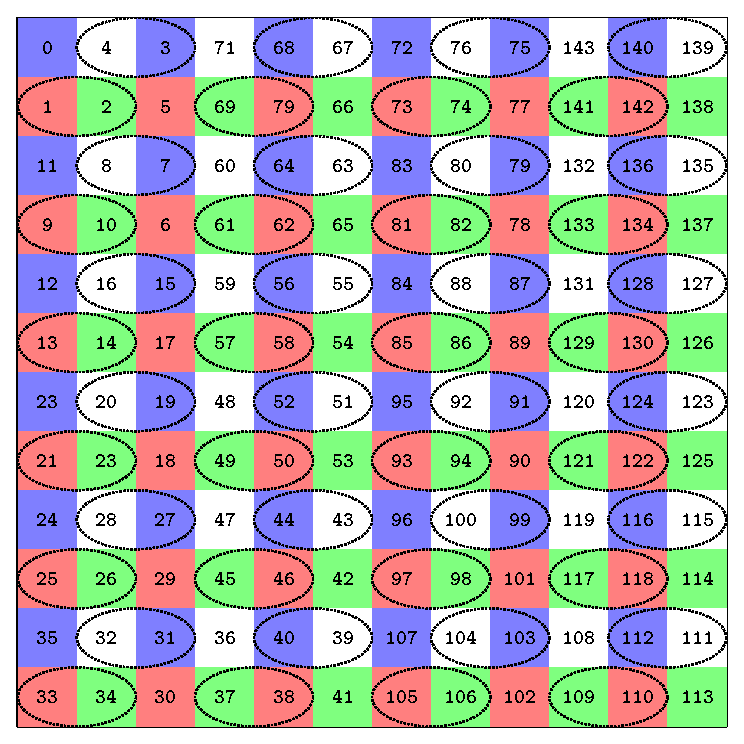
\includegraphics[scale=0.5]{reg}
\caption{An illustration of register bank allocation. The number in the cell is register number.
    The leftmost column registers are allocated to one block-column of $A$, the
topmost row registers are allocated to one block-row of $B$, and the others are registers for
a $12 \times 12$ sub-matrix $C$. Different colors denote the mapping of register banks as in Table~\ref{tab:ref}: green$\rightarrow$bank0,
blue$\rightarrow$bank1, gray$\rightarrow$bank2, red$\rightarrow$bank3.}
\label{fig:reg}
\end{center}
\end{figure}


\subsection{Memory Movement}
% According to the optimization observation on memory access suggested by microbenchmark,
According to our benchmarking observations, we use {\tt LDG.128} to load data from global memory through texture cache
and {\tt LDS.64} to load data from shared memory.
We also have additional reasons to adopt them in SGEMM kernel.
First, using {\tt LDG.128} reduces load instructions, hence reduce {\tt non-FFMA}s. %\jled{use load instead of non-FFMA. Use non-FFMA seems complicated.}
In the inner loop of Algorithm~\ref{gemm}, we need three {\tt LDG.128} instead of twelve {\tt LDS.32} to read twelve
words from $A$ column.
Second, the shared memory transaction size is 256 bytes, which forces each request being split into multiple transactions.
% it is another story for shared memory.
If we use {\tt LDS.128}, we can not infer the time of the second transaction by inspecting the inner loop, so it is
difficult to eliminate potential bank conflicts between {\tt LDS.128}s and {\tt FFMA}s.
However, it's determinable for {\tt LDS.64}, since a transaction just happens two cycles after the instruction is
issued. \jled{don't understand this sentence.}



\section{Evaluation}
\label{sec:experiment}


In this section, we compare the optimized SGEMM performance in Gflop/s with NVIDIA cuBLAS. 
Our SGEMM achieves $17\%\sim 25\%$ performance
improvement, which confirms the usefulness of the microarchitectural optimization on GPU. 
We present 
a quantitative analysis on the effect of each optimization strategy and an estimation of the upper bound performance using a roofline model.

The experiments are conducted on NVIDIA K20m GPU with its hardware configuration summarized in 
Table~\ref{table:k20}. We compare with cuBLAS from CUDA $7.0$. In our experiments, we choose square matrix for $A$, $B$
and $C$, and  the matrix sizes vary in $768\times768$, $1536\times1536$, $3072\times3072$, $6144\times6144$, $12288\times12288$.
%\jled{C size? What about A and B?}

\begin{table}[htbp]
\caption{The specification of NVIDIA Tesla K20m GPU.}
\centering
\scalebox{0.8} {
\begin{tabular}{|c|c|}
\hline
% Metric& Value\\
Configuration& Value\\
\hline
SPs/SM &192\\
\hline
SMs&13\\
\hline
Cores &2496\\
\hline
Frequency&705MHz\\
\hline
Memory Bus Width&320bit \\
\hline
Memory frequency&2600MHz\\
\hline
Bandwidth&208.0GB/s\\
\hline
Peak GFlop/s in SP&3520GFlop/s\\
\hline
Warp scheduler per SM&4\\
\hline
Dispatch unit/SM&8\\
\hline
Max Registers/thread&256 \\
\hline
    32-bit registers/SM&65536 \\ %\jled{Use actual number}\\
\hline
LD/ST unit&32 \\
\hline
shared memory size&48KB\\
\hline
L1 cache size&16KB or 48KB\\
\hline
L2 cache size&1536KB\\
\hline
\end{tabular}
}
\label{table:k20}
\end{table}


\subsection{Overall Performance}
Figure~\ref{fig:sgemm_tn} reports the performance of cuBLAS SGEMM and our optimized SGEMM.
When matrix size is $12288\times12288$, the optimized SGEMM achieves $3104$ GFlop/s with $88\%$ efficiency, while cuBLAS gets $2509$ GFlop/s with $71\%$ efficiency. 
Our SGEMM achieves $17\%$ performance improvement over cuBLAS.

The overall trend Figure~\ref{fig:sgemm_tn} is that SGEMM performance increases with matrix sizes. 
%\jled{the next sentence change to ``On the one hand, a larger matrix has a higher arithmetic intensity 9$AI$), which is the ratio of compulsory floating-point operations to the total DRAM memory traffic.
%The high arithmetic intensity makes good use of GPU computing resources to obtain good performance.''}
On the one hand, a large matrix has a high ratio of 
floating-point operations to the store operations of matrix $C$, which is more close to the hardware arithmetic intensity. 
On the other hand, a larger matrix has a better load balance on GPU by increasing the workload of the threading CUDA
cores.
%\jled{change to ``number of threading blocks''}. 
The number of threading blocks range in $4 \times 4, 8 \times 8, \dots, 64 \times 64$ from left to right in Figure~\ref{fig:sgemm_tn}.
% $[768/192,768/192]=[4,4]$ to $[12288/192, 12288/192]$ $=[64,64]$. 
Since Kepler has $13$ SMs in total, matrix $768\times 768$ suffers more from load imbalance because of only a few ($16$) blocks. 
This is why a significant performance growth from $768$ to $1536$ for SGEMM. 
With respect to performance improvement over cuBLAS, our optimizations benefits more on larger matrices. 
The higher arithmetic intensity of larger matrices makes their performance increasingly bounded by the GPU microarchitecture rather than memory. 
Therefore, our microarchitecture-level optimization plays an important role on tuning 
performance.

\begin{figure}[htbp]
\begin{center}
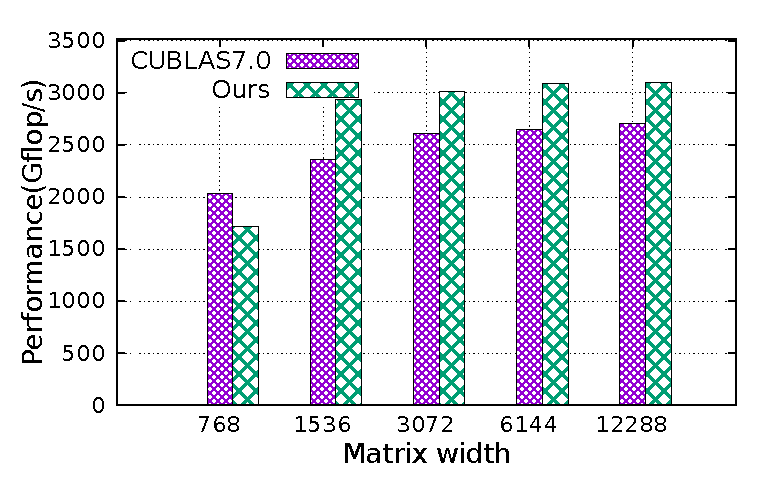
\includegraphics[scale=0.6]{sgemm_tn}
\caption{Performance comparison of CUBLAS and the optimized SGEMM }
\label{fig:sgemm_tn}
\end{center}
\end{figure}

\subsection{Performance Analysis}

\subsubsection{Register Blocking Size Influence}
Table~\ref{tab:dm} summarized computation and data movement volume of blocking SGEMM algorithm.
The volume of data moving from shared memory to global memory is $rx\times bk+ ry\times bk$, and computation volume is $rx\times ry\times bk$. 
The shared memory arithmetic intensity ($sAI$) is defined as the ratio of floating-point operations to the shared memory traffic, which is 
\begin{equation}
sAI = \frac {rx\times 
ry\times bk} {rx\times bk+ ry\times bk} = \frac{1}{\frac{1}{rx} + \frac{1}{ry}}.
\end{equation}
This function implies that larger register blocks get the higher shared memory arithmetic intensity.
The optimal solution should be in the case of $rx=ry$. %\jled{what about C is not square matrix?}. 
For global memory, we have a similar conclusion.%\jled{Add another equation for $AI$}

However, register blocking size is limited by number of registers per thread. 
%the maximum number of threads in one block.
In order to hide shared memory latency, double-buffered software pipelining is an efficient way. 
Each thread needs $rx\times ry$ registers to store the result of a sub-matrix of $C$, $rx$ and $ry$ registers to store a block-column of $A$ and a block-row of $B$ in the same loop. 
For double-buffering, extra $rx$ and $ry$ registers are used to prefetch next block-column of $A$ and block-row of $B$ from shared memory. 
Since the total number of registers must be less than the maximal number of registers per thread ($256$ on Kepler), we have
\begin{equation}
    rx\times ry + rx\times 2 + ry\times 2 < 256.
\label{f_register}
\end{equation}
Because data load must be aligned in $128$-bit using 
{\tt LDG.128}, the block size could be $4\times 4$, $8\times 8$ or $12\times 12$. 
Since $4\times 4$ leads to low data reuse in register files, Figure~\ref{fig:block} plots $8\times8$ and $12\times12$ cases.
We choose $12\times12$ over $8\times8$ because
$12\times12$ blocking has higher $sAI$ and instruction level parallelism. 
With respect to 
instruction scheduling optimization as Table~\ref{tab:position}, it has more slots to insert scheduling instructions,
making the {\tt LDS} overhead being more easily amortized. 
Thus, $12*12+4*12=192$ registers are used by {\tt LD} and {\tt FFMA} instructions, and totally $236$ registers with
other address indices.%\jled{what other?}.
The number of registers per SM restricts us to launch up to $256$ threads. 
In our implementation, we have $256$ threads per block. 
Each thread block computes a $192\times 192$ sub-matrix of $C$ by multiplying $A_{192,4}$ and $B_{4, 192}$, where $4$ is the unrolling factor.

\begin{figure}[htbp]
\begin{center}
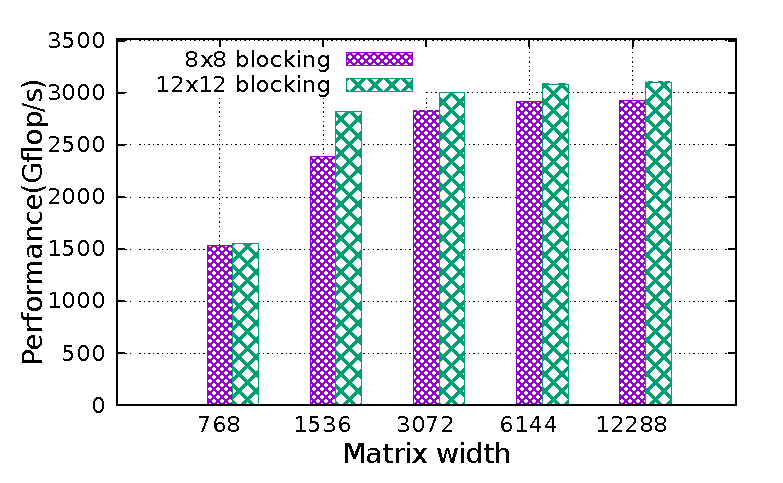
\includegraphics[scale=0.6]{block}
    \caption{Evaluation of different blocking sizes.} %\jled{could add $4\times4$ case.}}
\label{fig:block}
\end{center}
\end{figure}

Only one thread block per SM is active due to register limitation, thus the thread occupancy is $256/1024=12.5\%$.
With our high instruction level parallelism, the thread parallelism becomes low.
However, our SGEMM's high performance confirms that instruction level parallelism plays an more important role on GPU.
Similar conclusion is mentioned by Volkov in~\cite{volkov2010better}.

\subsubsection{Profiling Microarchitectural Optimization}

In order to examine performance gain of different optimization strategies, we construct several intermediate 
implementations by incrementally applying our microarchitectural optimizations.
\begin{figure}[htbp]
\begin{center}
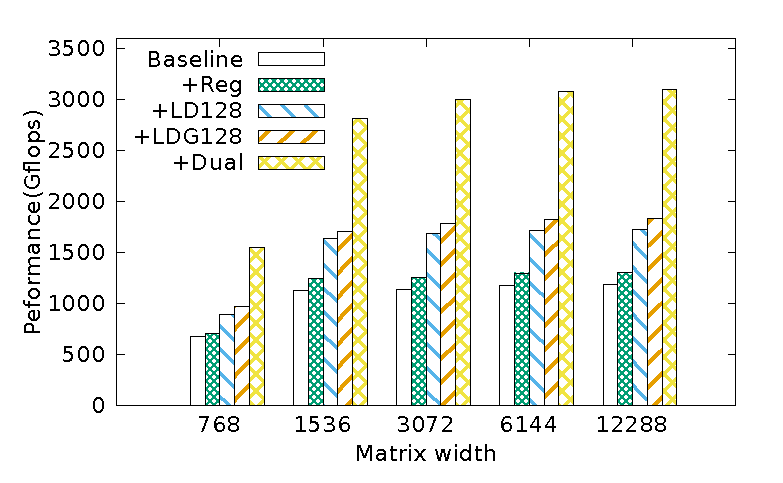
\includegraphics[scale=0.65]{tn_prof}
    \caption{Evaluation of the incremental optimizations.}
\label{fig:th_prof}
\end{center}
\end{figure}

{\it Baseline:}~~The baseline includes conventional optimizations including register blocking, global
memory double buffering, shared memory double buffering and unrolling, without assembly level optimization.
For example, the baseline uses default $32-bit$ {\tt LD} rather than $128-bit$ {\tt LDG} instruction to load data from global memory.
Registers is allocated orderly first for $C$, from $0$ to $143$, then for $A$ and $B$. 
In this case, {\tt FFMA}s have $368/(144*4)=63.89\%$ 2-way bank conflicts and $64/(144*4)=11.11\%$ 3-way bank conflicts. 
Besides, the baseline cannot apply dual issue optimization either.

{\it +Reg:}~~The register allocation pattern described in section~\ref{sec:register} is applied to eliminate register bank conflict. 
No optimization on instruction scheduling for this version.

{\it +LD128:}~~Use wider global load instruction {\tt LD128} with L2-cached.
Though Kepler has a L1 data cache, but it is designed for local rather than global memory access~\cite{gk110}.
% So {\tt LDx} will not be L1-cached, it can be L2-cached.

{\it +LDG128:}~~Use the texture cached {\tt LDG} which is faster than L2-cached {\tt LD}. 
When {\tt LDG} is used, {\tt TEXDEPBAR} is required before the data access due to weak consistence of texture cache~\cite{lukyanov2014efficient}.

{\it +Dual:}~~Use dual issue control, which is fully enabled by utilizing the pattern described in section~\ref{sec:assembler}.
%Single issue is controlled by setting control code to $0x40$. %\jled{different from section~\ref{sec:benchmark}. The left sentence is useless.}. 
For dual issued code, {\tt NOP} may be inserted for instruction alignment.

Figure~\ref{fig:th_prof} illustrates performance gains of each optimization method.
As long as the number of instructions is changed, rescheduling instruction order is needed to achieve good performance.
Compared to the baseline implementation, SGEMM gain up to $2.6\times$ speedup by applying all the optimization.
Register bank conflict eliminating improves around $10\%$ performance. 
Wider load instruction ({\tt LD128} improves $27\%-35\%$, texture cached
load instruction {\tt LDG128} improves $5\%-12\%$.
Dual issue improves the most, $84\%-106\%$.


\begin{figure}[htbp]
\begin{center}
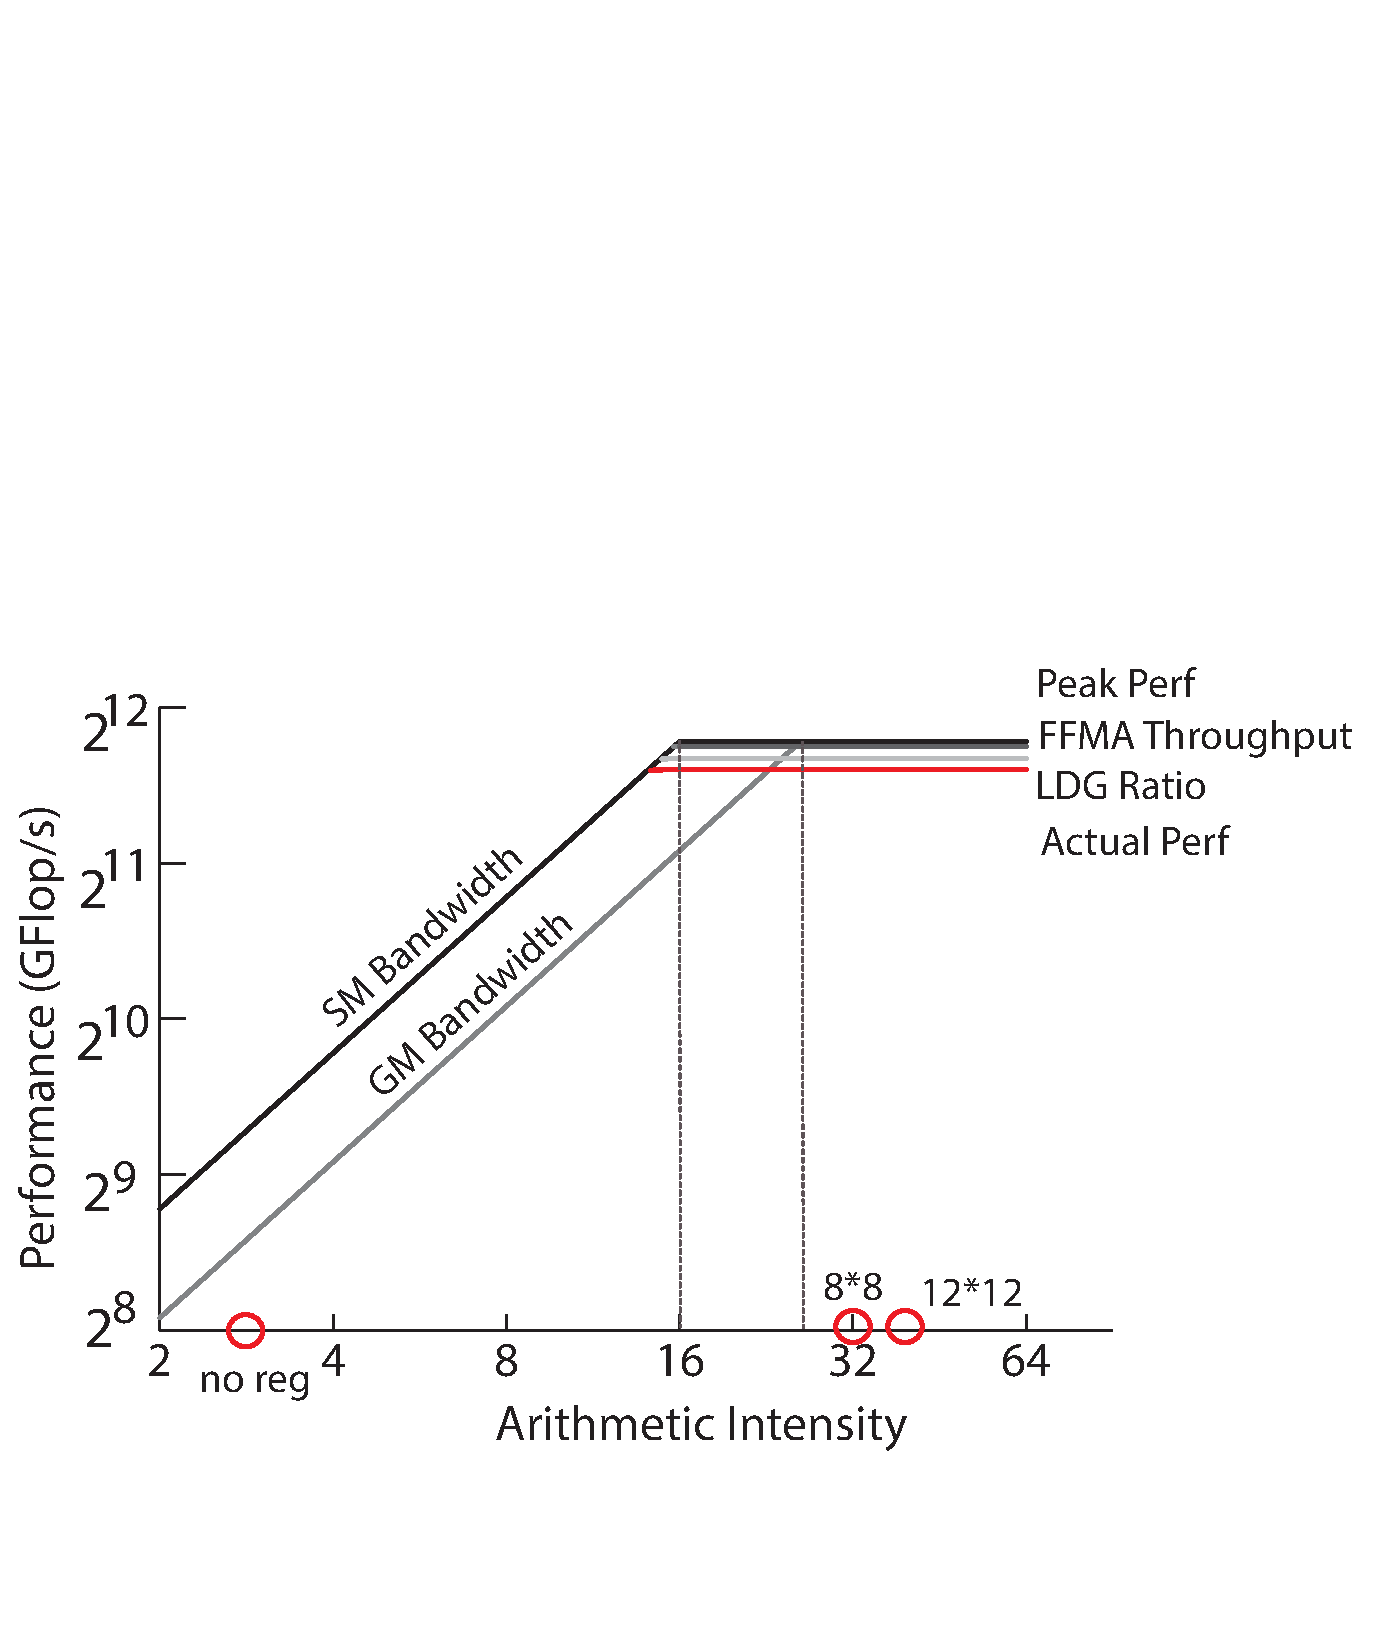
\includegraphics[scale=0.32]{roofline}
    \caption{Global memory roofline model using log-log scale. ``GM Bandwidth'' means global memory's theoretical bandwidth. Horizontal lines correspond to our incremental optimizations.}
\label{fig:roofline_global}
\end{center}
\end{figure}

\begin{figure}[htbp]
\begin{center}
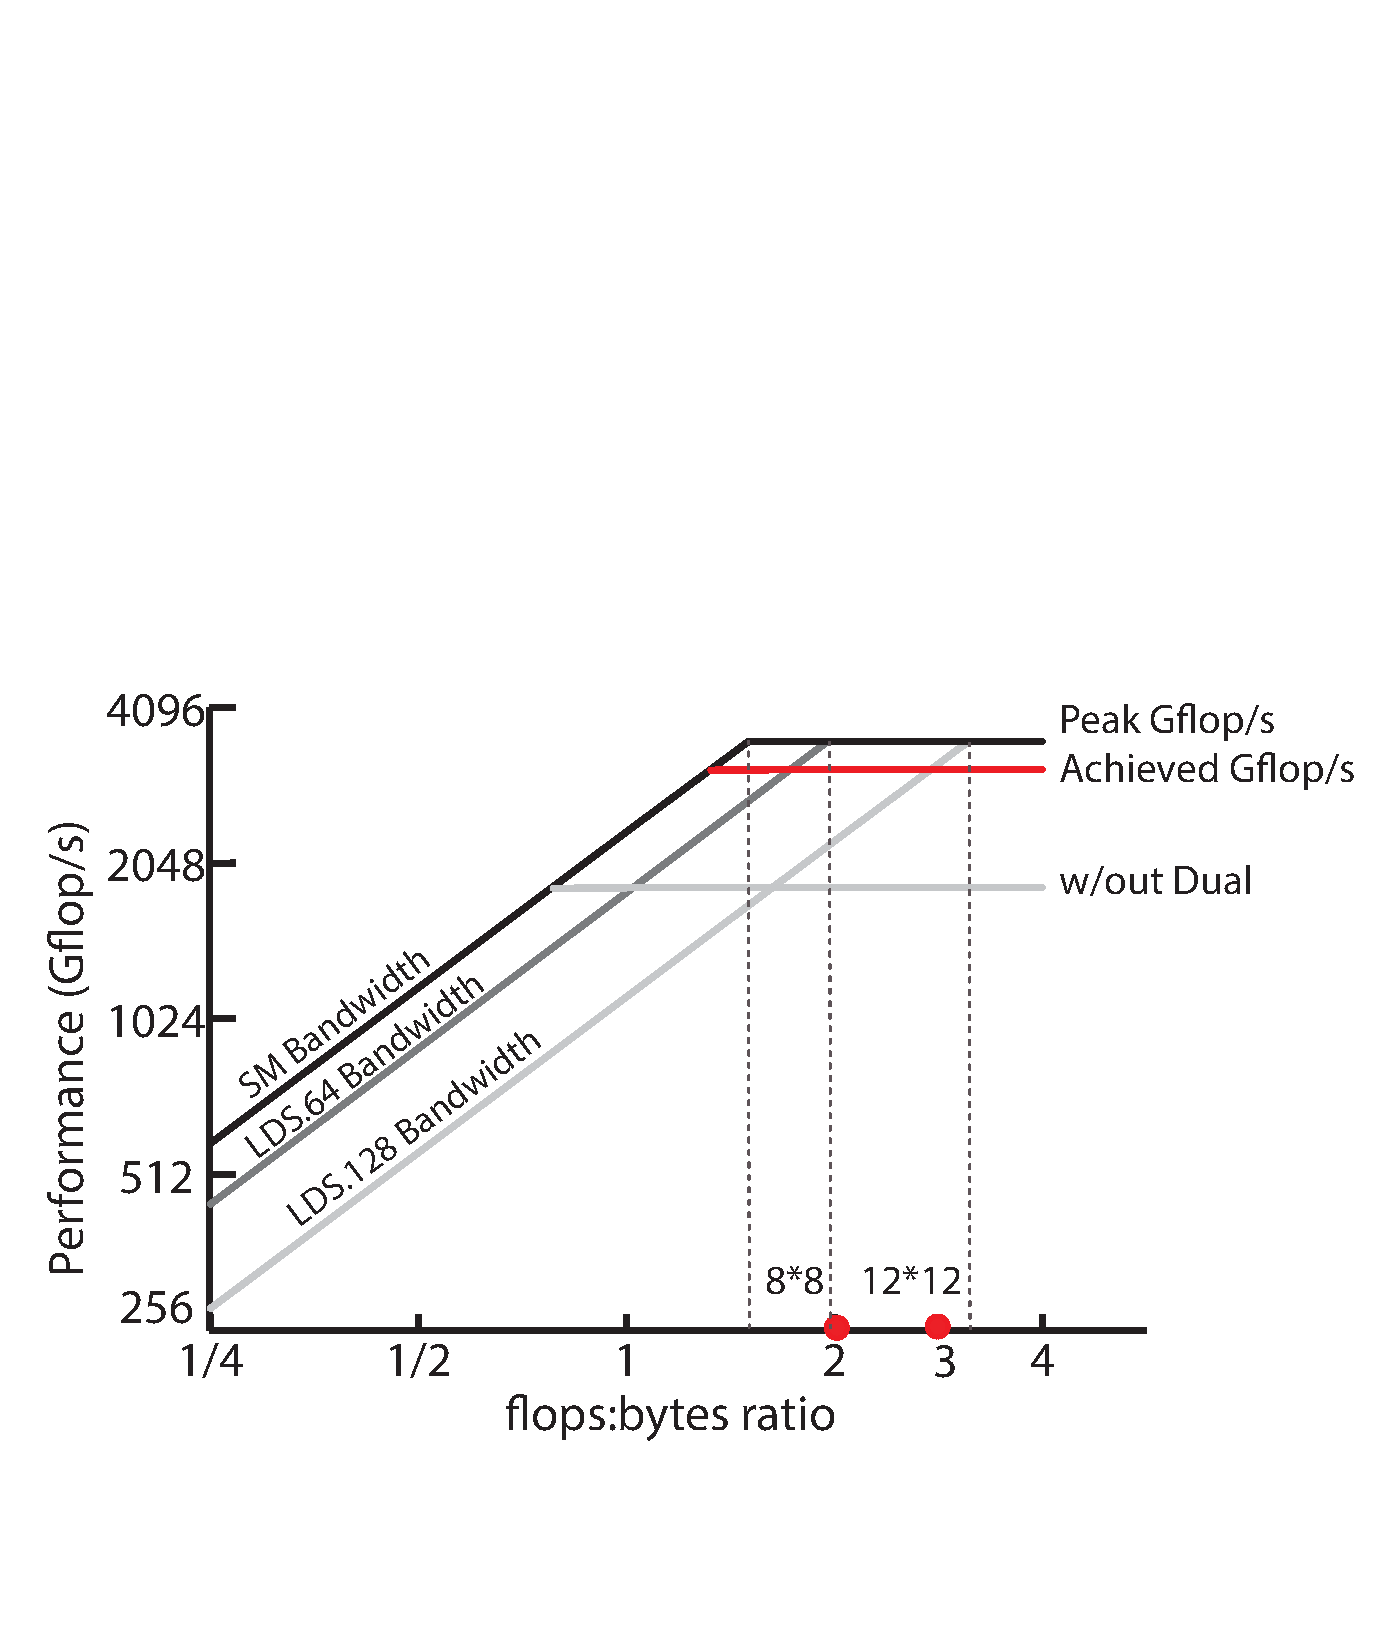
\includegraphics[scale=0.32]{roofline_sm}
    \caption{Shared memory roofline model using log-log scale. ``SM Bandwidth'' means shared memory's theoretical bandwidth. Horizontal lines correspond to our incremental optimizations.}
\label{fig:roofline_shared}
\end{center}
\end{figure}

\subsubsection{Upper Bound Analysis}


We estimate the upper bound factors: {\tt LDS}, {\tt LDG} and {\tt FFMA} which correspond to three kinds of resources, 
shared
memory, global memory, and computation power. In register blocking loop, each thread computes $bm*bn*bk$and reads $bm*bk+bn*bk$ words. The upper bound of global memory bandwidth can be modeled as:
\begin{displaymath}
    \frac{2*bm*bn*bk}{4*(bm*bk + bn*bk)} = \frac{Gflop/s}{bandwidth}
\end{displaymath}
According to parameters in our SGEMM implementation, $bm=bn=192$, $bk=4$, $Gflop/s=3520$, so $73$ GB/s is the minimal
requirement for global memory bandwidth in order to achieve peak $3520$ Gflops.
For shared memory, inside each loop, $(rx*bk + ry * bk)*tx*ty$ words will be read from shared memory, in which $tx$,
$ty$ is block dimension, $rx$, $ry$ is register blocking size. The computation is $bm*bn*bk$. Based on the ratio of computation to shared memory access,
\begin{displaymath}
    \frac{2*bm*bk*bn}{4*tx*ty*(rx*bk + ry *bk)}  = \frac{Gflop/s}{bandwidth}
\end{displaymath}


For Kepler GPU the minimum bandwidth requirement for shared memory is $1173$GB/s, and the bandwidth requirement is
$1173/13=90$ GB/s for each SM. The hardware can provide $200$GB/s global memory bandwidth and $2349$GB/s shared memory bandwidth in
theory, which is higher than requirement, and hence neither bandwidth of shared width nor global memory will be bottleneck.

SGEMM has different computation to memory ratio in terms of  global memory and shared memory, so we draw two roofline models. 
The slope of slash lines in Figure~\ref{fig:roofline_global} is bandwidth of global memory. The x-axis is computation to global
memory access ratio of an application. For SGEMM, by $12\times12$, the ratio is $48$, by $8\times 8$ blocking, the ratio
is $32$. The horizontal black lines corresponding to our {\tt FFMA} throughput optimization which including elimanating
register banks, choosing proper load width. Our SGEMM currently achieves at the red line. This figure demonstrates that
by $12\times12$ blocking, SGEMM is not global memory bounded.
The slope of slash lines in Figure~\ref{fig:roofline_shared} is bandwidth of shared memory. The x-axis is computation to
shared memory access ratio of an application. For SGEMM, by $12\times12$, the ratio is $3$, by $8\times 8$ blocking, the ratio is $2$. 
This figure shows by our optimization,  SGEMM will not be bounded by shared memory. However, if we use {\tt LDS.128} instead of
{\tt LDS.64}, even $12\times 12$ blocking, SGEMM will be bounded by shared memory.



The loss to peak performance can be explained as the following reasons. As we have shown in 
Section~\ref{sec:assembler}, {\tt FFMA} throughput can achieve $97.67\%$. The loss is about $2.33\%$, which may comes 
from overhead of warp scheduler in {\tt FFMA} dual issue mode. The double-buffering algorithm can amortize the latency 
of {\tt LDS}.
With $12x12$ register blocking and $4$ times unrolling, there will be $144*4=576$ {\tt FFMA} instructions in the loop.
With our designed {\tt FFMA} dual issue pattern, every $6$ {\tt FFMA} needs $4$ clock cycles in the pipeline.
It needs $4*144*4/6=384$ clock cycles for each thread,  two $128$ bits {\tt LDG} instruction are needed.
We observe each {\tt LDG} has $10$ clock penalty, the total {\tt LDG} will cause $2*10/384 = 5.2\%$ loss. Other penalty 
comes from synchronization and writing $C$ matrix in the block.






\section{Related Work}
\label{sec:related}
%To our knowledge, this paper provides the first comprehensive study of demystifying NVIDIA GPU microarchitecture which 
%is correlated with performance tuning in SGEMM. 
This section briefly discusses related work in reverse engineering ISA encoding, GPU assembler, microbenchmarking and SGEMM optimization.

{\em {\bf ISA Encoding Solver and GPU Assembler}}:The lack of assembler for public use motivates a series of work on developing toolchains to facilitate tuning codes in 
assembly level. 
For the early architecture G80, Decuda~\cite{decuda} demonstrated the feasibility to operate
assembly instructions. After that, for almost each new generation of CUDA architecture, there are several 
efforts on developing assembly toolchains. Both Hou's Asfermi~\cite{asfermi} and Bernstein's 
cudaasm-qhasm~\cite{bernstein2012usable} are assemblers for Fermi architecture. Gray built MaxAs~\cite{maxas} assembler 
for Maxwell architecture by reverse engineering the encoding of Maxwell GPU. 
Although Envytools~\cite{envytools} supports translation of PTX instruction to $64$-bit binaries 
for serval GPU architectures, it is not able to generate a compatible {\tt cubin} format which can be directly used by 
the CUDA driver APIs. %Besides, no prior work presents the detailed instruction decoding algorithms process as ours.
It's no doubt that all their work envolves reverse engineering GPU ISA
encodings. However, neither detailed descriptions are given nor a general tool is developed to crack
new GPU ISA encoding. We provide a general tool to crack different GPU ISA encoding
automatically, and a complete assembler for Kepler architecture.
%A remarkable advantage of our assembly toolchain is the compatibility with CUDA's {\tt cuobjdump}. 

%We share the same idea of performance microbenchmarking with other works. 
{\em {\bf Benchmarking}}: Wong et.al.~\cite{wong} performed a 
comprehensive benchmarking work on GT200 and provided pipeline latency data and
memory features. Mei~\cite{mei} benchmarked memory hierarchy including cache, shared memory on Fermi, Kepler and Maxwell GPU.
However, neither of them benchmarked 
vectorized load instructions like {\tt LD} and {\tt LDS}. 
%Due to lack of considering vectorized load instructions and 
%too less instructions inside the loop, the results is not so accurate.
No vectorized load instructions are benchmarked and too few instructions inside the loop lead to results with unsatisfying accuracy.
Neither of them considered dual issue mode of 
arithmetic instructions. We leverage the complete assembler to crack control codes which reveal more 
microarchitecture details for tuning application performance.

{\em {\bf Matrix Multiplication Tuning}}: With respect to GEMM optimization in microarchitectural level, some work inspires our implementation 
on specific GPUs. For example, we adopt the proved effective optimization techniques like shared memory/register 
blocking and double-buffering~\cite{volkov}~\cite{tan}. Further, Tan et.al.~\cite{tan} implemented fast DGEMM by using 
assembly level optimization, such as software pipelining, vector memory operations, and instruction scheduling. 
Lai~\cite{lai} presented performance analysis and optimization work of SGEMM on both Fermi and GTX680 GPUs. However, 
Lai didn't consider dual issue mode by setting control code, which can boost performance significantly. Scott 
Gray~\cite{nervana_sgemm_wiki} presented optimization of SGEMM in assembly on Maxwell GPU. Since Maxwell does not 
support {\tt FFMA} dual issue, the optimization is not as complex as 
Kepler. In contrast, we present a complete case of applying microarchitectural features by combining 
register allocation, dual issuing, memory access paths and instruction scheduling.

\section{Conclusion}
\label{sec:conclusion}
We have presented a methodology to demystify GPU's microarchitecture level optimizations and demonstrated its applicatio
n to tune SGEMM. The methodology relies on a reverse engineering approach to crack the instruction encoding of GPU archi
tecture, and a profound microbenchmarking at assembly level to correlate architecture features with performance factors,
 such as dual issue impact on float arithmetic throughput, memory load width on bandwidth, register bank distribution on
 performance etc. These parameters are worthwhile for both hardware and software researcher to understand how GPU archit
ecture is designed and how to adapt program to GPU hardware. As far as we know, it is the first time to provide a detail
ed description of how we cracked the instruction encoding by presenting the decoding solver. This solver is not limited 
to Kepler GPU, it can be used to crack the future GPU encoding automatically.

Based on these disclosed information, we implemented the fastest SGEMM on Kepler GPU. The optimized SGEMM is $3104$ Gflo
p/s and efficiency is $88\%$, CUBLAS's SGEMM achieves $2509$ Gflp/s ($71\%$ efficiency). Our optimized one is $17\%$ hig
her than Cublas. The performance boost is achieved on the basis of tuning {\tt FFMA} throughput as high as hardware peak
, then add other non-FFMA instruction with little penalty. These optimizations include register bank conflict eliminatin
g, {\tt FFMA} dual issue scheduling, choosing proper width of global load and shared memory load instructions and so on.
 Our work opens a door to optimize NVIDIA GPU code at native machine level. The development of GPU compiler could learn 
experiences from these microarchitectural-level optimizations.


%
% The following two commands are all you need in the
% initial runs of your .tex file to
% produce the bibliography for the citations in your paper.
%\bibliographystyle{abbrvnat}
\bibliographystyle{plain}

% The bibliography should be embedded for final submission.

\bibliography{bib/ref}

\end{document}

%                       Revision History
%                       -------- -------
%  Date         Person  Ver.    Change
%  ----         ------  ----    ------

%  2013.06.29   TU      0.1--4  comments on permission/copyright notices
